\documentclass[fleqn,10pt]{physiome}
% Use option lineno for line numbers 
\usepackage{adjustbox}
\usepackage{makecell}
\usepackage{float}
\usepackage{hyperref}
\usepackage{url}
\articletype{Original}
%% Choose from Original, Retrospective, Review, Letter

\title{Computational Modelling of Glucose Uptake in the Enterocyte}

\author[1][nima.afshar@auckland.ac.nz]{Nima Afshar}
\author[1]{Soroush Safaei}
\author[1]{David P. Nickerson}
\author[1]{Peter J. Hunter}
\author[1,2]{Vinod Suresh}
\affil[1]{Auckland Bioengineering Institute, University of Auckland,New Zealand}
\affil[2]{Department of Engineering Science, University of Auckland,New Zealand}

%% The following lines can be omitted when submitting;
%% information will be added by editors
\publicationdate{1 October 2020}
\editor{Karin Lundengård}
\curator{Anand Rampadarath}
\submitteddate{30 September 2020}
\accepteddate{1 October 2020}
\citethisas{Afshar et al. (2020)\\ Computational Modelling of Glucose Uptake in the Enterocyte. Physiome.}{10.36903/physiome.13034423}
\begin{document}

\maketitle

\begin{abstract}
We describe an implemented model of glucose absorption in the enterocyte, as previously published by \cite{afshar2019computational}, The model used mechanistic descriptions of all the responsible transporters and was built in the CellML framework. It was validated against published experimental data and implemented in a modular structure which allows each individual transporter to be edited independently from the other transport protein models. The composite model was then used to study the role of the sodium-glucose
cotransporter (SGLT1) and the glucose transporter type 2 (GLUT2), along with the requirement for the existence of the apical Glut2 transporter, especially in the presence of high luminal glucose loads, in order to enhance the absorption. Here we demonstrate the reproduction of the figures in the original paper by using the associated model.
\end{abstract}

\keywords{PHYSIOME, CellML, OpenCOR, Computational modeling, Glucose uptake}

\primarypubs[10.36903/physiome.13034423]{sample}{afshar2019computational}

\section{Introduction}

In the primary paper, a validated computational model was proposed for explaining glucose uptake from intestinal lumen into epithelial cell. The main goal of this paper is to show that the figures in the primary paper can be reproduced by using the correlated model in the PMR. Results from the model were compared with experimental results from \citet{zheng2012mechanisms} which studied the glucose uptake on two different cell lines - Caco2 and IEC6 - by using varying concentration of glucose (0.5 - 50 mM).
Here we introduce a quick instruction to reproduce each figure in the original paper. 

\section{Model description}

We present a mathematical model that includes apical GLUT2 and is parameterised against published experimental data, and was used to study the contributions of SGLT1 and GLUT2 in published cell culture data on glucose uptake \citep{zheng2012mechanisms}. The implemented model used mechanistic models of all relevant transporters. In particular, we replaced the Na-Cl co-transporter in the original model with individual models for the anion
exchanger 1 (AE1) and Na$^+$/H$^+$ exchanger (NHE3) proteins at the apical
membrane and incorporated ENaC and CFTR channels for apical Na$^+$ and Cl$^-$ transport.
This makes it possible to use the model to study scenarios where the
expression and/or function of these transport proteins is altered, for example
in gene knockout/mutation studies or in the use of channel inhibitors and agonists. We constructed a mathematical model of the epithelial cell of a small intestine (enterocyte) that incorporates the relevant transport proteins identified in the
literature \citep{barrett2015electrolyte} and diffusion pathways (\autoref{fig.1}). The
membrane localisation and function of these transporters and the source of the
original mathematical models are listed in \autoref{Table 1}.\newline

\begin{figure}[H]
\centering
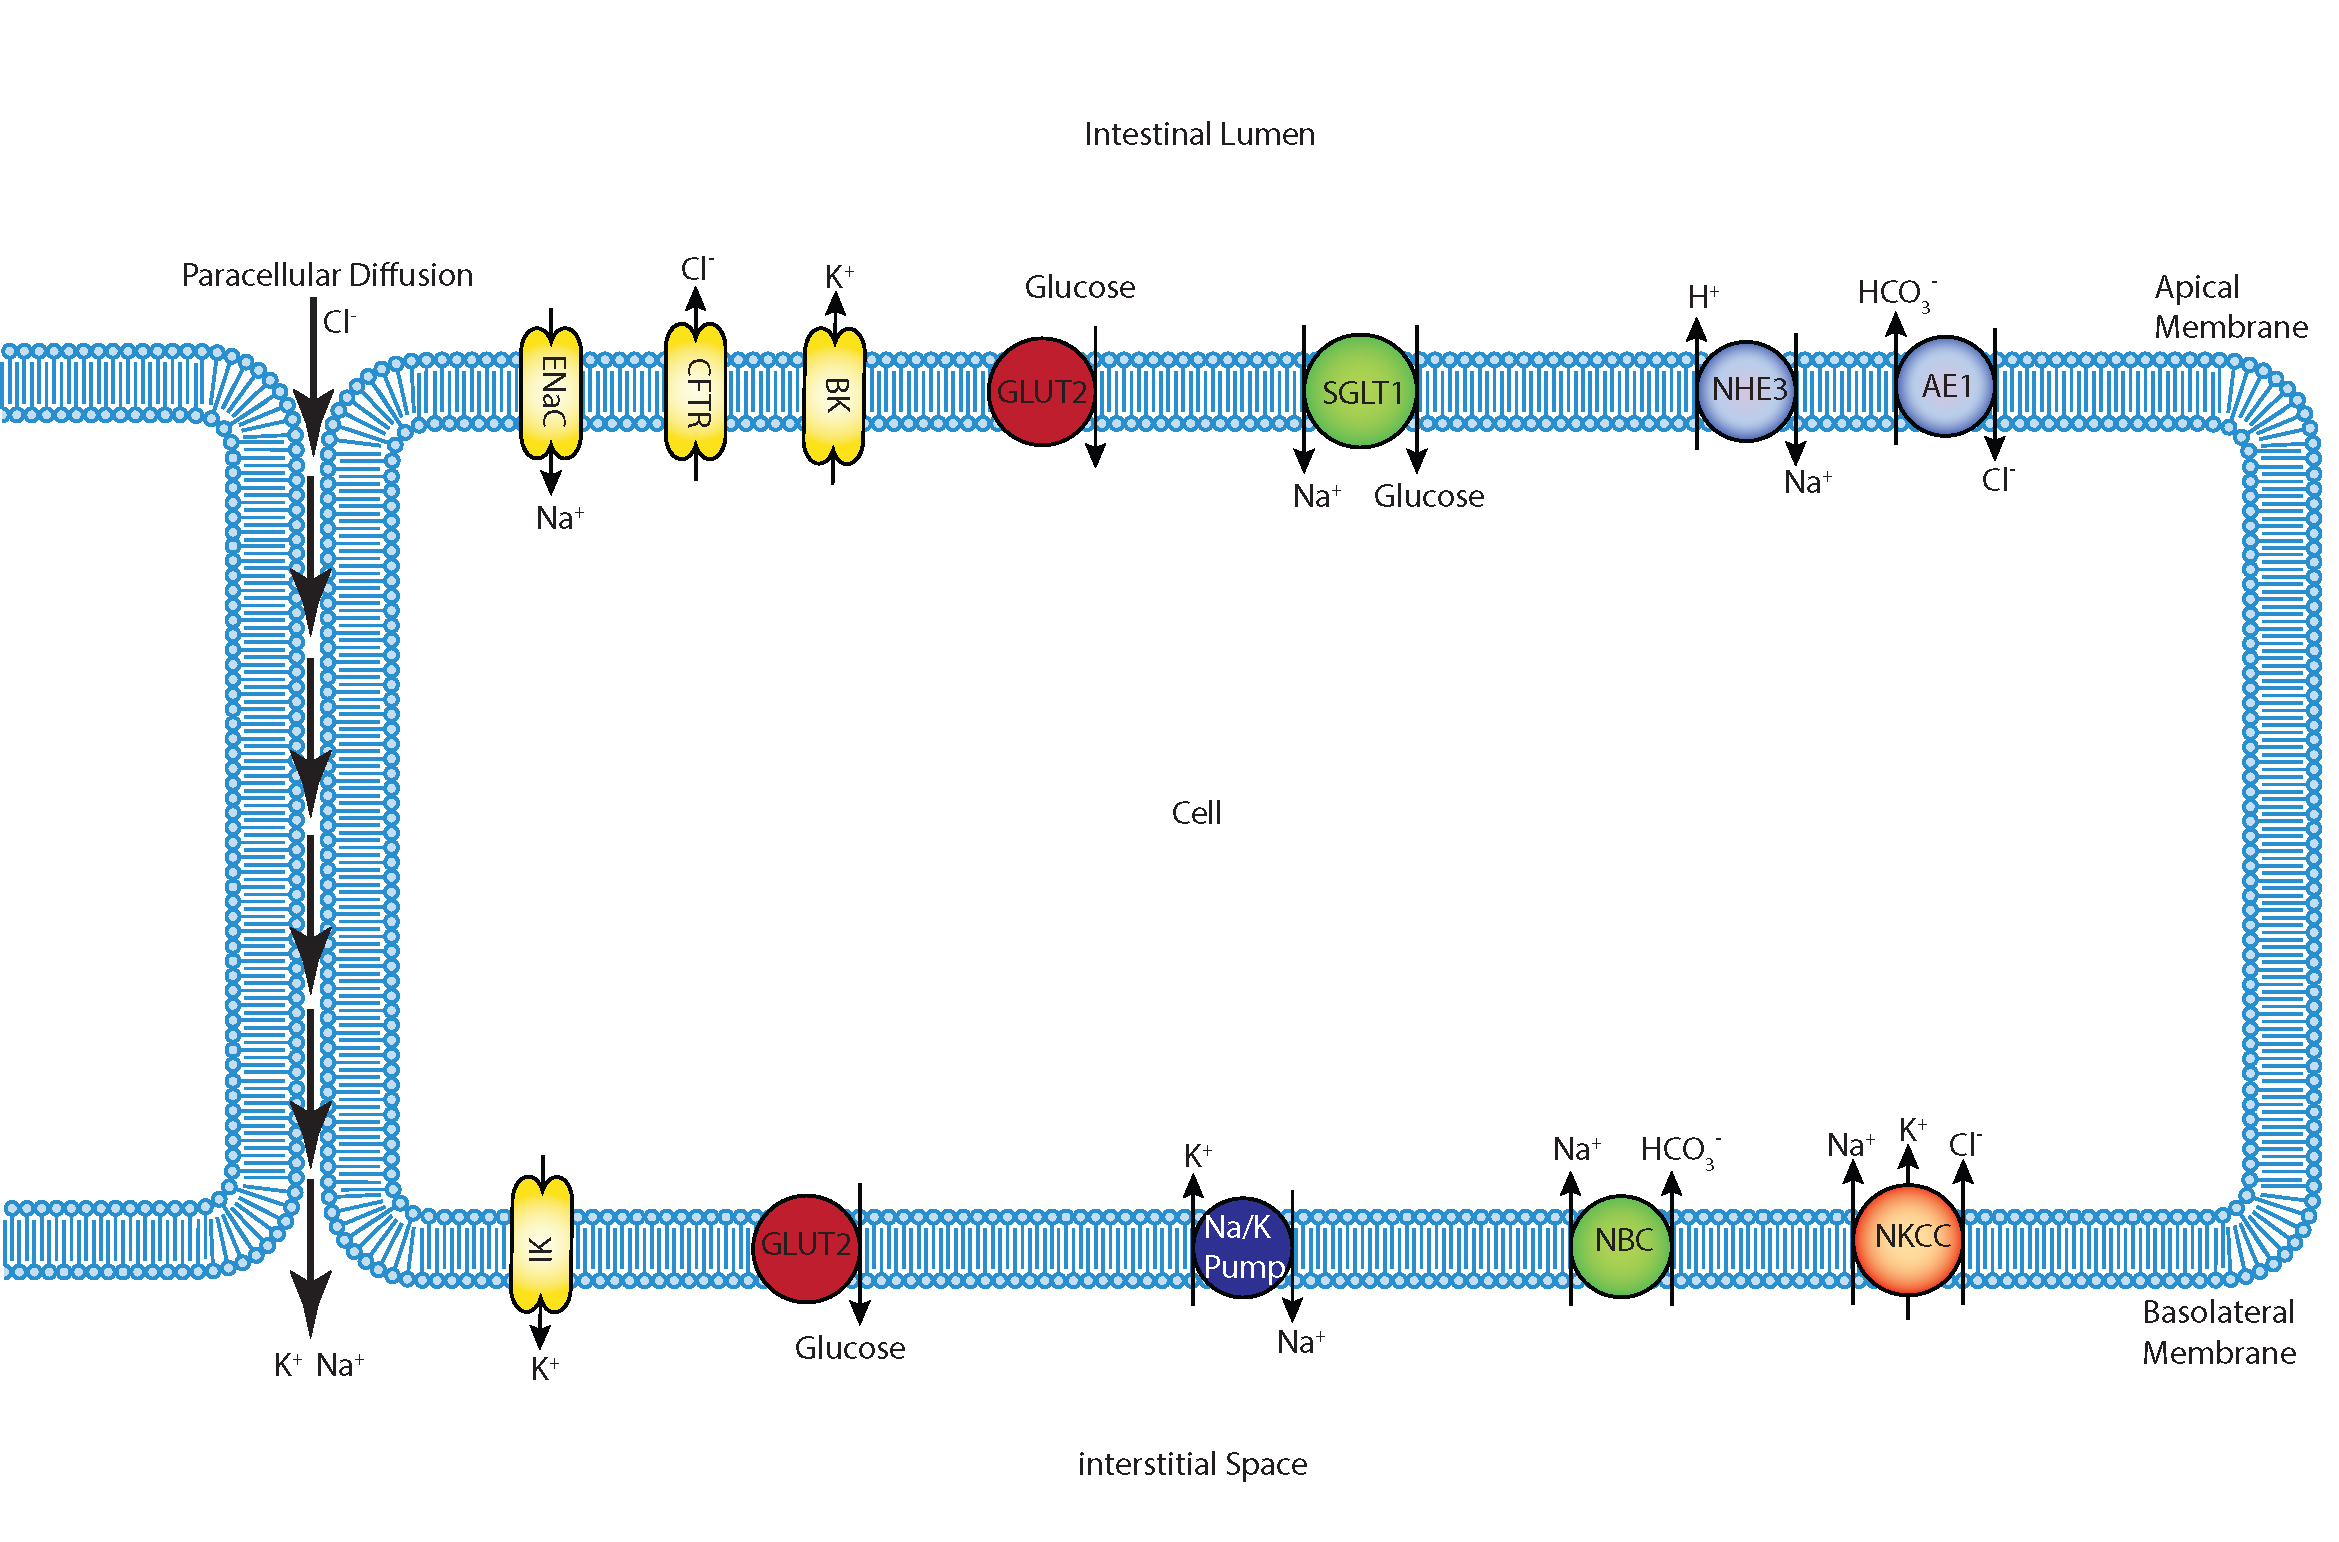
\includegraphics[width=0.85\linewidth]{fig01.jpg}
\caption{Schematic of enterocyte showing the relevant
transporters in the apical and basolateral membrane along with
the apical (lumen) and basolateral (interstitium) extracellular
domains.}
\label{fig.1}
\end{figure}\newline


The apical (luminal) and
basolateral (interstitial) surface of the cell are in contact with distinct extracellular
compartments. Transport of substances occurs across the membranes as
well as directly between the extracellular compartments across the paracellular
junctions. The variables to be solved in the model are chemical species (${Na^+}$,
${K^+}$, ${H^+}$, ${Cl^-}$, ${HCO_3^-}$, glucose) concentrations in each compartment and the
two membrane potentials. Flux balance and electric charge conservation laws
yield the governing equations of the model. Water transport is not included and
hence we limit ourselves to modelling iso-osmotic transport.\newline


\begin{table}[ht!]
	\centering
	\onecolumn
	\caption{\label{Table 1} List of transporters used in the model along with their locations and roles}
	\begin{adjustbox}{width=1\textwidth}
		\begin{tabular}{|c|c|c|c|c|}
			\hline
			Transporter& Location & Role & Chemical Species & \makecell{Source of the\\mathematical model} \\
			\hline
			SGLT1& Apical & Cotransporter &  1 Glucose, 2 $Na^{+}$ & \cite{parent1992electrogenic}\\
			\hline
			NaK ATPase& Basolateral & 
			Exchange Pump & 3$Na^{+}$, 2$K^{+}$ & \cite{thorsen2014transepithelial}\\
			\hline
			GLUT2&\makecell{Apical and Basolateral} & Uniporter Protein  &  Glucose & \cite{pradhan2013carrier}\\
			\hline
			NHE3& Apical& Antiporter & 1 $Na^{+}$, 1 $H^{+}$ & \cite{weinstein1995kinetically}\\
			\hline
			AE1&Apical & Antiporter & 1 $Cl^{-}$, 1 $HCO_{3}^{-}$ & \cite{weinstein2000mathematical}\\
			\hline
			BK& Apical& Channel & $K^{+}$ & \cite{fong2016computational}\\
			\hline
			CFTR&Apical &  Channel &  $Cl^{-}$ & \cite{fong2016computational} \\
			\hline    
			CLC-2&Basolateral &  Channel &  $Cl^{-}$ & \cite{fong2016computational} \\
			\hline     
			ENaC&Apical & Channel & $Na^{+}$ &  \cite{fong2016computational} \\
			\hline
			IK & Basolateral & Channel & $K^{+}$ & \cite{fong2016computational} \\
			\hline
			NBC& Basolateral & Cotransporter  & 1 $Na^{+}$, 3 $HCO_{3}^{-}$ & \cite{ostby2009astrocytic} \\ 
			\hline
			NKCC1& Basolateral & Cotransporter & 1 $Na^{+}$, 1 $K^{+}$, 2 $Cl^{-}$ &  \cite{palk2010dynamic}\\
			\hline  
		\end{tabular}
	\end{adjustbox}
\end{table}\newpage

The model is implemented in the open source, extensible markup language
(XML)-based CellML modelling environment used to represent mathematical
models of biology based on ordinary differential and algebraic equations \citep{cuellar2003overview}. We adopted a modular, compositional approach to model
construction by reusing CellML models of individual transport proteins encoded
in an online, curated repository (Physiome Model Repository (PMR,
models.physiomeproject.org)) to facilitate the sharing of models \citep{yu2011physiome}. All simulation were run using OpenCOR (Version 0.5) \citep{garny2015opencor}.
All results presented here can be reproduced using the SED-ML or Python scripts noted in the figure captions. In some cases the simulation results are saved to CSV files for plotting using a Python script also noted in the figure caption. We used python 3.6 with the following versions of different libraries: numpy 1.17.4, matplotlib 3.1.2, pandas 0.25.3, scipy 1.3.3.

The original CellML file along with all the codes can be found in the following link in the PMR:\newline

\url{https://models.physiomeproject.org/workspace/572}\newline\newline

\section{Model results}
\textit{Dynamic response to an apical glucose stimulus}\newline

In these simulations, the compositions of the apical and basolateral compartments were identical
and held constant (140 mM Na+, 5.4 mM K+, 103 mM ${Cl^-}$). A time dependant, extracellular glucose stimulus was applied at t = 60 s (\autoref{fig02}A). The simulation file \href{https://models.physiomeproject.org/workspace/572/file/057757b3a8de9a56b4bd32b8a12a0f00af1d8213/SEDML_files/Fig02.sedml}{Fig02.sedml} contains the computational setting for running the model.\newline

\begin{figure}[ht]
\centering
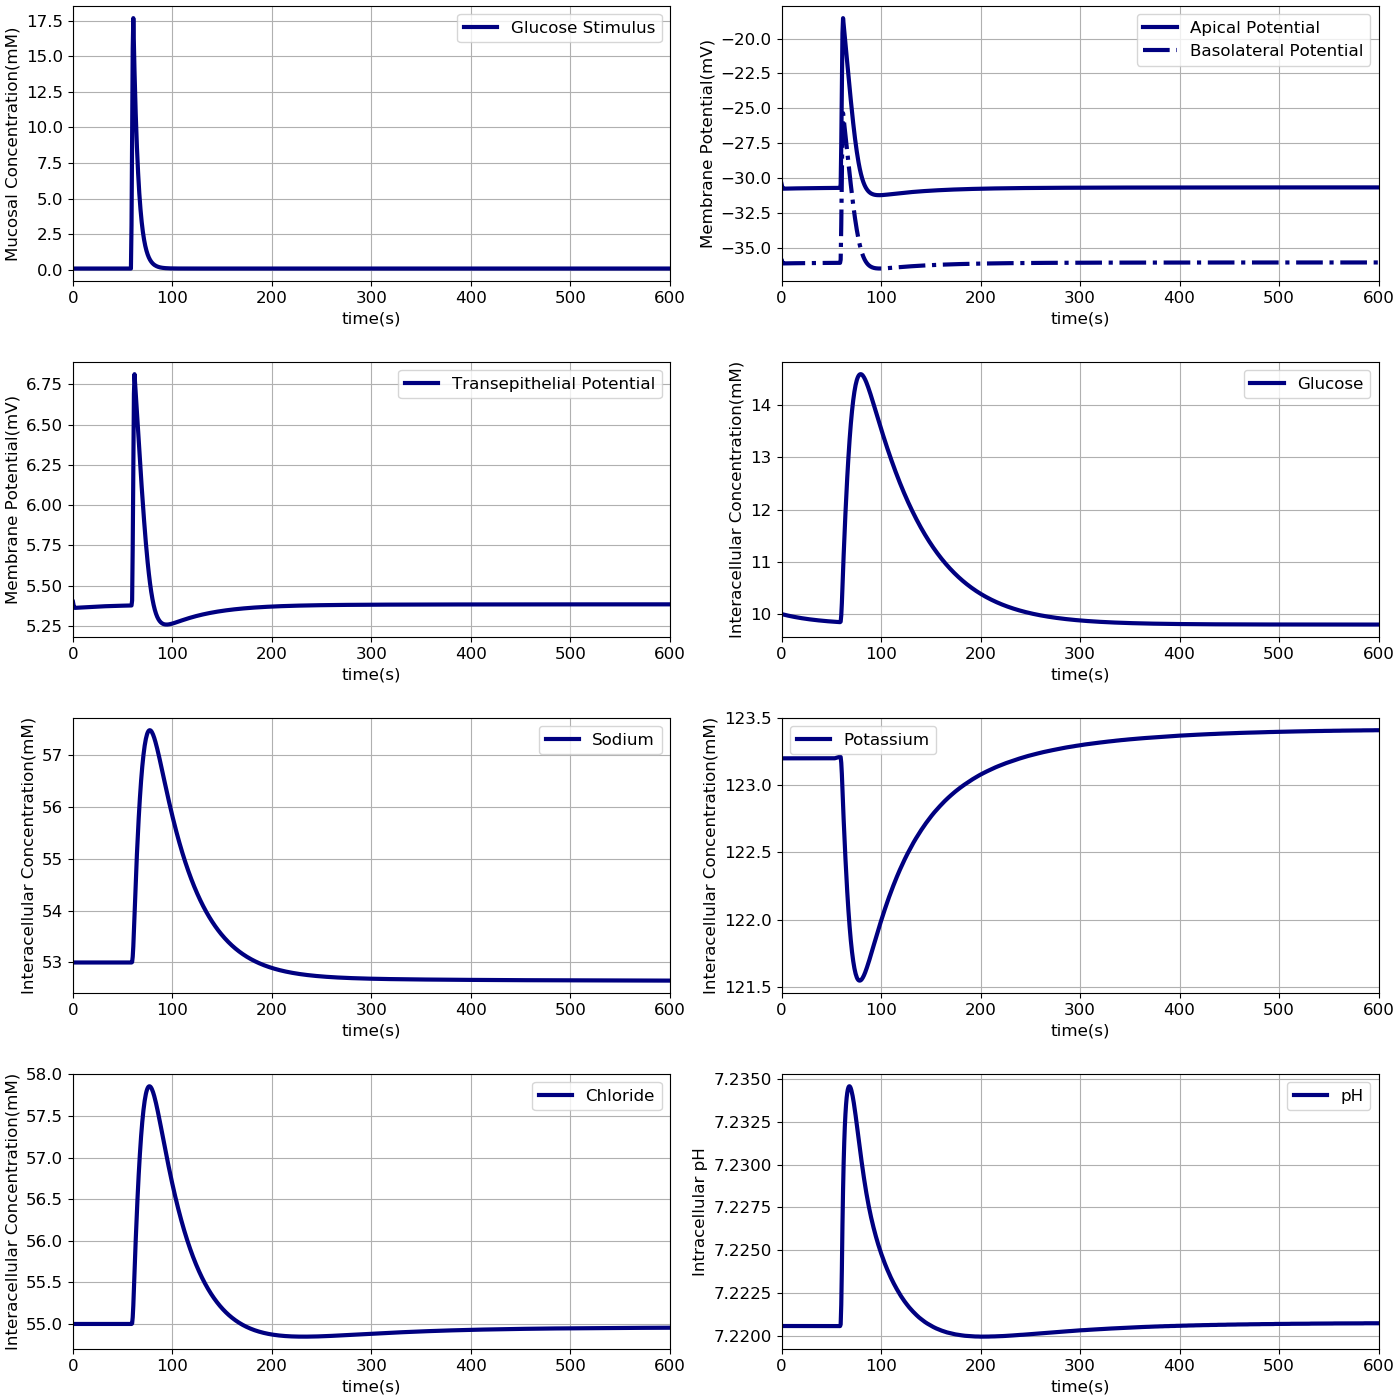
\includegraphics[width=0.8\linewidth]{fig02.png}
\caption{Dynamic response of the model to an extracellular
glucose stimulus. The stimulus consists of: A - a step increase
followed by an exponential decay.B - Apical and basolateral
membrane potentials, C - transepithelial potential, D -and intracellular
concentrations of glucose, E - sodium, F - potassium, G - chloride and H - pH are shown. The results presented in the \autoref{fig02} can be reproduced with the \href{https://models.physiomeproject.org/workspace/572/file/59488c15178b09bcb5b11f795383b1435f7b7ef1/SEDML_files/Fig02.sedml}{Fig02.sedml} in OpenCOR}
\label{fig02}
\end{figure}

\textit{Comparison with the \cite{thorsen2014transepithelial} model}\newline

In the next step the results from our model were compared to results from Thorsen model under the same condition. Model outputs were normalised against the steady state values of the Thorsen model and are shown in \autoref{fig03}. We implemented the Thorsen model in CellML which can be found in the PMR link \footnote{\url{https://models.physiomeproject.org/workspace/5b8}}. All the values in our model are normalised against the corresponding steady-state values in the Thorsen model as described in the python script. \newpage

\begin{figure}[ht]
\centering
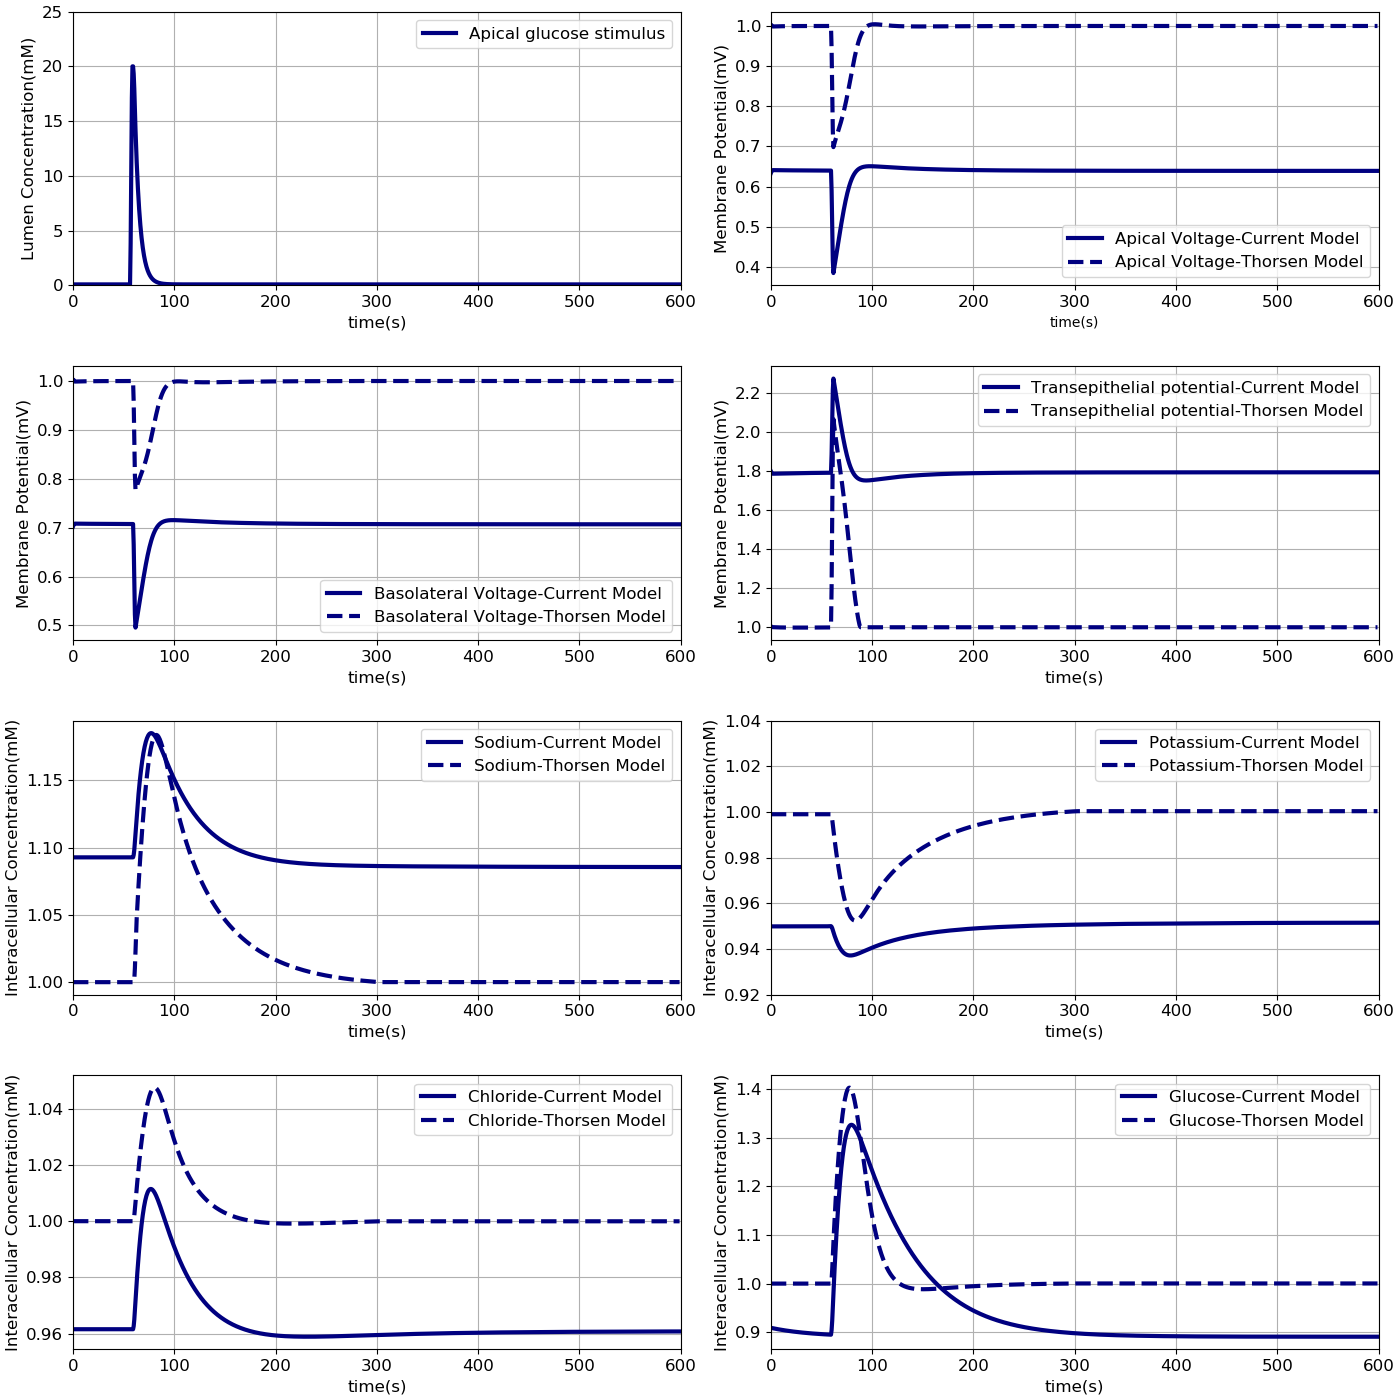
\includegraphics[width=0.8\linewidth]{fig03.png}
\caption{Comparison of model responses against the model
of Thorsen et al (2014). Each variable has been normalised
against the corresponding steady value from the Thorsen model. The results presented in the \autoref{fig03} can be reproduced with the \href{https://models.physiomeproject.org/workspace/572/file/59488c15178b09bcb5b11f795383b1435f7b7ef1/SEDML_files/Fig03.py}{Fig03.py} script in OpenCOR and \href{https://models.physiomeproject.org/workspace/572/file/59488c15178b09bcb5b11f795383b1435f7b7ef1/SEDML_files/Fig03-plot.py}{Fig03-plot.py} script}
\label{fig03}
\end{figure}

\textit{Comparison against cell culture data}\newline

Finally, model predictions were compared against measurements carried out in
cell culture studies \citep{zheng2012mechanisms}. The experiments used Caco-2 and
IEC6 cell lines. While Caco-2 expresses both SGLT1 and GLUT2, IEC6 cells
do not express GLUT2. We therefore turned off the expression of GLUT2 in
the apical membranes to simulate these cells(in component "Cell\_Concentration", {$\theta_{26}$}=0). To measure glucose uptake, varying concentrations (0.5 -- 50 mM) of glucose were introduced into the apical chamber in a buffer solution with a baseline composition of $130$ mM NaCl, $4$ mM KH$_2$PO$_4$, $1$ mM CaCl$_2$. The osmolarity of the buffer was maintained during the measurements by modulating the NaCl content such that if the glucose concentration was $x$ mM, NaCl concentration was $130 - x/2$ mM. After exposure to the glucose stimulus for different durations (30 -- 600 $s$), cells were lysed and intracellular glucose and protein concentrations were measured. Since the measurements were reported in nanomole glucose per milligram (mg) protein, the data were converted to concentration units (millimole per litre, mM) by doing the unit conversion from nanomole/$m^{3}$ to mM and also multiplying by the cellular protein concentration (mg protein per ml cell volume). The conversion factor $a$ (protein density) was used as a fitting parameter in a non-linear Generalized Reduced Gradient optimization to match model outputs to the data. The optimization  was done using the Microsoft Excel Solver (Microsoft Office 2013) by minimizing the least square error between model predicted and measured intracellular glucose concentration.These results indicate that the model is able to reproduce a range of independent experimental observations.
The volume of the basolateral compartment ($V_b$) was fixed at different multiples ($m$ = 0.1, 1, 10) of the cell volume ($V_c$) and also as an infinite bath to generate a range of predictions. This allowed us to account for the uncertainty in the actual volume of the basolateral compartment, we collected a range of model predictions by varying the parameter from small (0.1 times the cell volume) to large (an infinite compartment) values (\autoref{fig04}).\newline

\begin{figure}[ht]
\centering
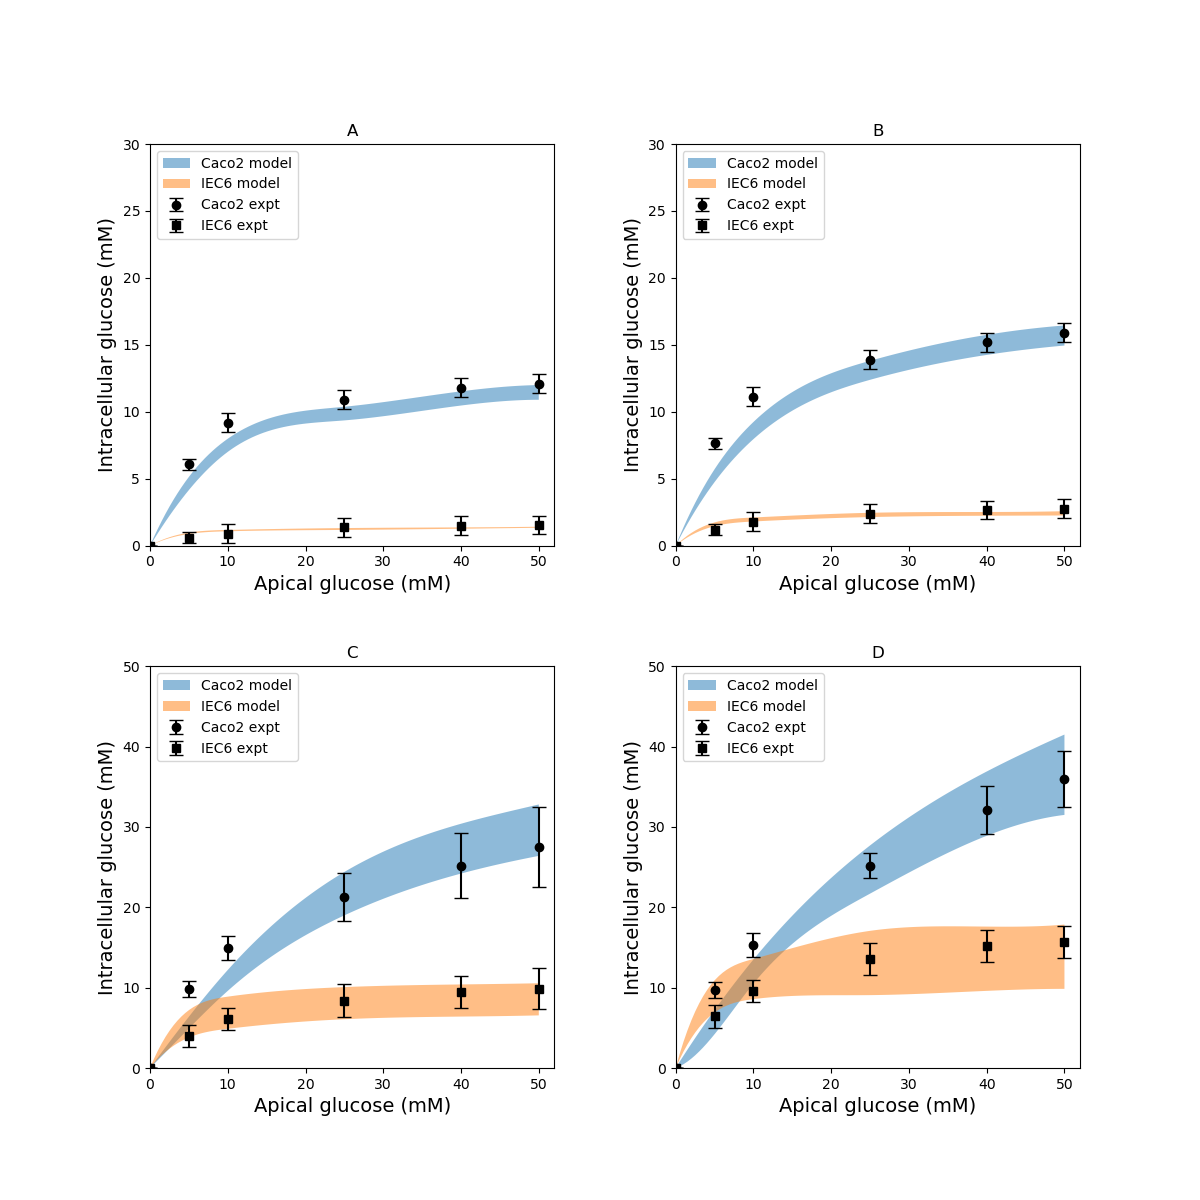
\includegraphics[width=0.9\linewidth]{fig04.png}
\caption{Intracellular glucose concentrations for a range of extracellular glucose concentrations in Caco2 and IEC6 cells and exposure times (A: 30 s, B: 60 s, C: 300 s, D: 600 s). Experimental data points and error bars were digitally extracted from Zheng et al (2012). Strips for the model predictions represent the range of values generated by setting $V_b = m V_c, m = 0.1, 1, 10, \infty$. The results presented in the \autoref{fig04} can be reproduced with the \href{https://models.physiomeproject.org/workspace/572/file/c052b0c460280139dad150937fbee4fa6a026505/SEDML_files/Fig04.py}{Fig04.py} script in OpenCOR and \href{https://models.physiomeproject.org/workspace/572/file/c052b0c460280139dad150937fbee4fa6a026505/SEDML_files/Fig04_plot.py}{Fig04-plot.py} script}
\label{fig04}
\end{figure}\newline

\textit{Role of apical GLUT2 in glucose uptake}\newline

In the original study of Zheng et al, the experimental data in \autoref{fig04}
were interpreted as indicating the presence of GLUT2-mediated uptake at the
apical membrane \citep{zheng2012mechanisms}. In \autoref{fig05} we investigated whether an alternative explanation
was possible whereby SGLT1 expression levels in the model could be
tuned to reproduce the same trends in intracellular glucose concentration. In
\autoref{fig05}, the data for Caco-2 cells at the 600 s time point are compared
to the model with varying levels of apical GLUT2 and SGLT1. The baseline
model with normal expression of SGLT1 and apical GLUT2 provides a good fit
to the data over the full range of apical glucose concentrations (\autoref{fig05}A). 
When apical GLUT2 is turned off (in component "Cell\_Concentration", {$\theta_{26}$}=0) with no changes in SGLT1 expression (Figure
\ref{fig05}B), model predictions of intracellular glucose are low compared to the
data for apical glucose concentrations higher than 10 mM. In addition, model
predictions saturate after around 20 mM of apical glucose while the data shows
an increasing trend. A higher expression of SGLT1 was also examined and can
provide a better match to the data in the absence of apical GLUT2. With
no apical GLUT2 and 2-fold levels of baseline SGLT1 (\autoref{fig05}C) the model
overpredicts the data at low apical glucose concentrations (< 10 mM) and underpredicts
the data at apical glucose concentrations > 40 mM (in component "SGLT1\_Flux", $n_{SGLT}$ $\times$ $2$). When SGLT1 levels are increased to 3 times the baseline value (in component "SGLT1\_Flux", $n_{SGLT}$ $\times$ $3$), the model overpredicts the data over the whole range, except at an apical glucose of 50 mM (\autoref{fig05}D)

\begin{figure}[ht]
\centering
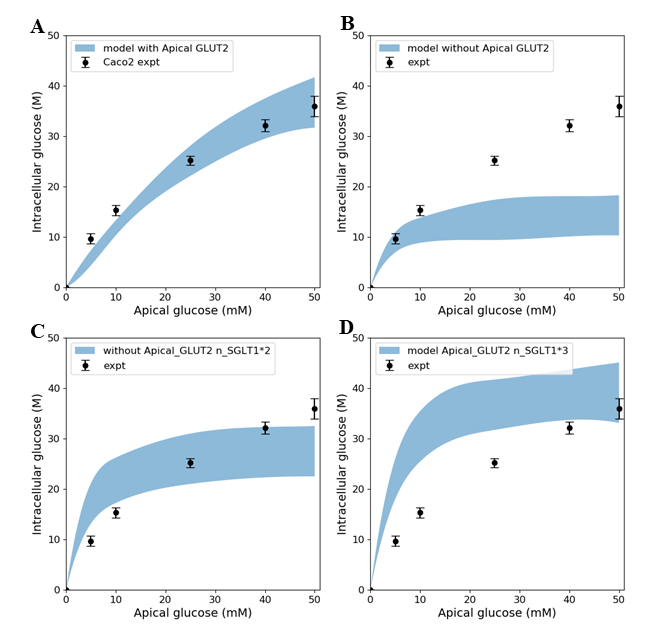
\includegraphics[width=0.8\linewidth]{fig05.png}
\caption{Intracellular glucose concentration versus extracellular glucose concentration in Caco2 in the presence/absence of Apical GLUT2 with different numbers of SGLT1 transporter A - Output of model with apical GLUT2 B - Model does not have apical GLUT2 C - Model does not have apical GLUT2 and the number of SGLT1 is doubled D -  Model does not have apical GLUT2 and the number of SGLT1 is 3-fold higher. Experimental data points and error bars were digitally extracted from Zheng et al (2012). Strips for the model predictions represent the range of values generated by setting $V_b = m V_c, m = 0.1, 1, 10, \infty$. The results presented in the \autoref{fig05} can be reproduced with the \href{https://models.physiomeproject.org/workspace/572/file/c052b0c460280139dad150937fbee4fa6a026505/SEDML_files/Fig05.py}{Fig05.py} script in OpenCOR and \href{https://models.physiomeproject.org/workspace/572/file/c052b0c460280139dad150937fbee4fa6a026505/SEDML_files/Fig05_plot.py}{Fig05-plot.py} script}
\label{fig05}
\end{figure}

The contribution of SGLT1 and GLUT2 to the apical glucose flux is shown in \autoref{fig06} following 600 s of exposure to apical glucose. The figure shows SGLT1 flux (where in component "Cell\_Concentration", {$\theta_{26}$}=0), GLUT2 flux (where in "Cell\_Concentration", {$\theta_{6}$}=0) and the total flux which is basically SGLT1 flux + GLUT2 flux. For different glucose loads in the lumen, the concentration of ions needs to be changed as described for \autoref{fig04}.\newpage

\begin{figure}[ht]
\centering
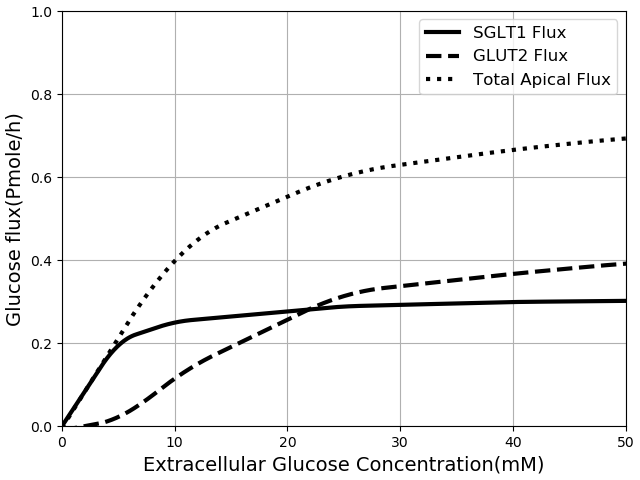
\includegraphics[width=0.7\linewidth]{fig06.png}
\caption{Glucose Flux through SGLT1 and GLUT2 in $600$ seconds of simulation along with total apical flux of glucose. The results presented in the \autoref{fig06} can be reproduced with the \href{https://models.physiomeproject.org/workspace/572/file/c052b0c460280139dad150937fbee4fa6a026505/SEDML_files/Fig06.py}{Fig06.py} script in OpenCOR and \href{https://models.physiomeproject.org/workspace/572/file/c052b0c460280139dad150937fbee4fa6a026505/SEDML_files/Fig06_plot.py}{Fig06-plot.py} script}
\label{fig06}
\end{figure}

The developed model was then used to study the effect of 3-fold elevated SGLT1 and GLUT2 expression levels on glucose flux into the basolateral compartment. \autoref{fig07} shows the ratio of steady state glucose flux into the basolateral compartment, normalised to the flux at baseline conditions over a range of apical glucose concentrations. In green line the number of SGLT1 protein was multiplied by 3 (in component "SGLT1\_Flux", $n_{SGLT}$ $\times$ $3$) and in blue line the number of GLUT2 transporter in both membranes was tripled (in component "A\_GLUT" and "GLUT2", $n_{GLUT}$ $\times$ $3$) and in red line both the SGLT1 and GLUT2 protein were increased 3-fold. For different apical glucose concentrations, other ion concentrations should be changed as described for \autoref{fig04}. All the values for each set were divided by the basolateral flux values from baseline conditions.\newpage

We developed a computational model of glucose transport in the enterocyte that includes the full set of relevant transporters. The model is able to reproduce measurements reported in the literature and can be used to answer physiologically relevant questions about glucose uptake rates and mechanisms. In addition, the capabilities of the CellML framework were exploited to compose existing validated models of individual transporters to create the final model, which provides greater confidence in the implementation and facilitates model reuse and sharing.
\begin{figure}[H]
\centering
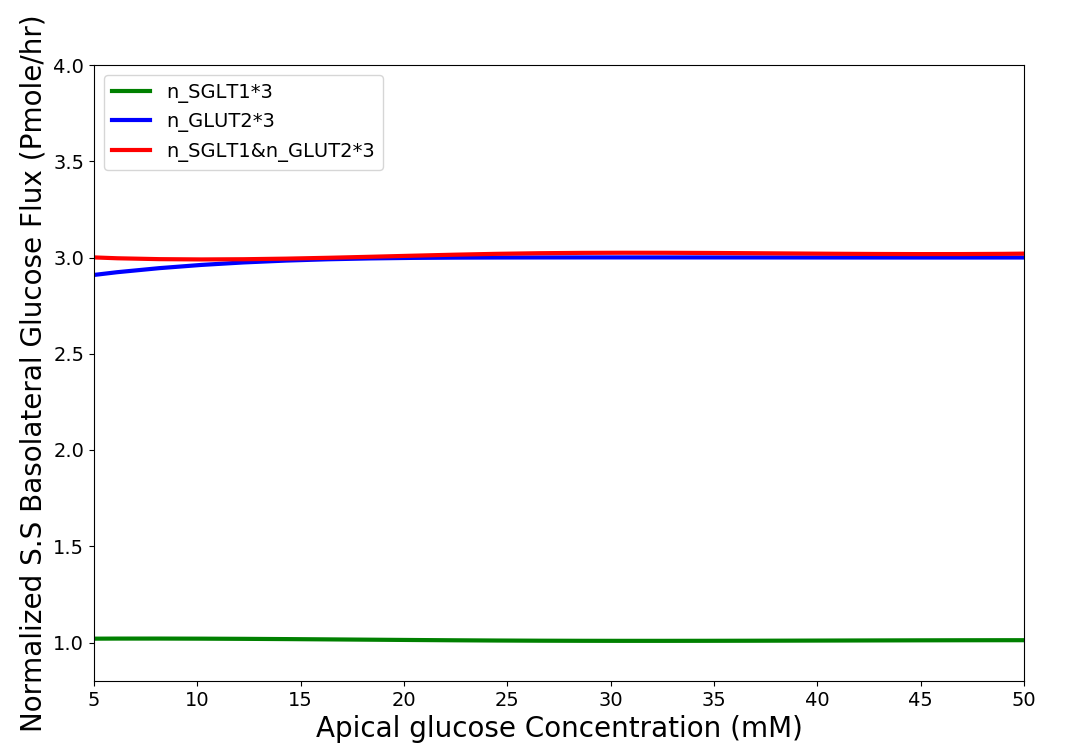
\includegraphics[width=0.8\linewidth]{fig07.png}
\caption{Normalised steady state basolateral glucose flux versus different stimulus of glucose in the  lumen when  number of SGLT1 is 3 fold higher(green), number of GLUT2  is 3 fold higher(blue) and number of both SGLT1 \& GLUT2 are 3 fold higher(red). The results presented in the \autoref{fig07} can be reproduced with the \href{https://models.physiomeproject.org/workspace/572/file/c052b0c460280139dad150937fbee4fa6a026505/SEDML_files/Fig07.py}{Fig07.py} script in OpenCOR and \href{https://models.physiomeproject.org/workspace/572/file/c052b0c460280139dad150937fbee4fa6a026505/SEDML_files/Fig07_plot.py}{Fig07-plot.py} script}
\label{fig07}
\end{figure}

\section{Discussion}

\textit{Comparison with existing models}\newline

Our model differs from the Thorsen et al. model \citep{thorsen2014transepithelial} in some
important respects. One of the differences between the two models is in the
treatment of sodium and chloride transport at the apical membrane. Thorsen
et al postulate electro neutral one-for-one fluxes of these ions to account for the
sodium-hydrogen (NHE3) and chloride-bicarbonate (AE1) exchangers and use
Goldman-Hodgkin-Katz (GHK) diffusion to model ENaC and CFTR. In contrast,
our model takes a more general approach by incorporating the individual
transport pathways at the apical membrane (\autoref{fig.1}). We examined the
implications of these modelling choices in \autoref{fig08}. \autoref{fig08}A shows the
ratio of the AE1 flux to NHE3 flux for the simulation conditions of \autoref{fig03}.
In the Thorsen model this ratio is equal to 1, whereas the ratio lies in the range
7 - 8 in our model. File \href{https://models.physiomeproject.org/workspace/572/file/057757b3a8de9a56b4bd32b8a12a0f00af1d8213/SEDML_files/Fig02.sedml}{Fig02.sedml} was run in the OpenCOR in order to plot chloride flux through AE1 over sodium flux via NHE3. $J\_{NHE3}\_{Na}$ and $J\_{AE1}\_{Cl}$ were plotted and all the data points in AE1 were divided by corresponding value in the NHE3 data set. Cl/Na cotransporter ratio as stated in the paper is equal to 1. Thorsen et al. used sodium and chloride diffusion through both apical and basolateral membrane of the cell. We replaced them with ENaC and CFTR transporters for sodium and chloride flux in the apical membrane respectively. \autoref{fig08}B shows the ratio of sodium and chloride flux through transporters in our model to the sodium and chloride flux through diffusion in the Thorsen model.\newline

\begin{figure}[ht]
\centering
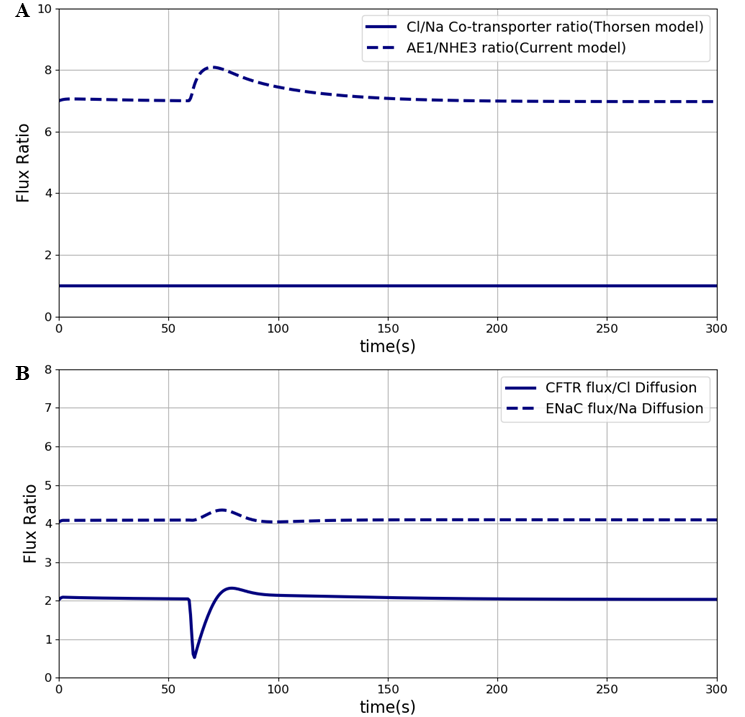
\includegraphics[width=0.75\linewidth]{fig08.png}
\caption{Sodium flux and Chloride flux through NHE3 and AE1 compare to NaCl co-transporter flux in the Thorsen model. The results presented in the \autoref{fig08} can be reproduced with the \href{https://models.physiomeproject.org/workspace/572/file/c052b0c460280139dad150937fbee4fa6a026505/SEDML_files/Fig08.py}{Fig08.py} script in OpenCOR and \href{https://models.physiomeproject.org/workspace/572/file/c052b0c460280139dad150937fbee4fa6a026505/SEDML_files/Fig08_plot.py}{Fig08-plot.py}}
\label{fig08}
\end{figure}\newpage

\autoref{fig09} shows the model output in each cell line separately. They both were plotted at different exposure times which indicates that over a short time (30 and 60 seconds) both the cell lines have tendency to level off. Over a longer time (>= 300 seconds) IEC6 still has a tendency to be saturated but in Caco2 glucose uptake keeps increasing in higher luminal glucose. \autoref{fig09} is another way to show \autoref{fig04} however it does not contain the experimental results by having all the exposure times for specific cell lines in one panel. Once again, strips for the model predictions represent the range of values generated by setting $V_b = m V_c, m = 0.1, 1, 10, \infty$. In this paper we described how each graph was plotted in the original paper to make things easier for other scientists in this area to become familiar with the entire process. We also showed that the primary model can be reproduced which may be a useful feature in generating other related models or expanding the current model.

\begin{figure}[ht]
	\begin{center}
		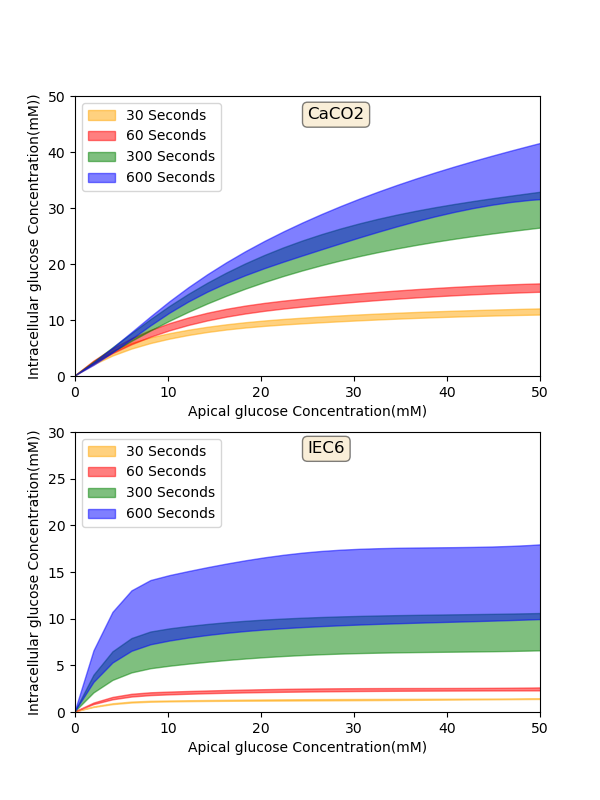
\includegraphics[scale=0.7]{fig09.png}
		\caption{\label{fig09} Model output - Intracellular glucose concentration versus Extracellular glucose concentration in a) Caco2 cell line and b) IEC6 cell line. The results presented in the \autoref{fig08} can be reproduced with the \href{https://models.physiomeproject.org/workspace/572/file/c052b0c460280139dad150937fbee4fa6a026505/SEDML_files/Fig09.py}{Fig09.py} script in OpenCOR and \href{https://models.physiomeproject.org/workspace/572/file/c052b0c460280139dad150937fbee4fa6a026505/SEDML_files/Fig09_plot.py}{Fig09-plot.py}}
	\end{center}
\end{figure}\newpage


\bibliography{sample}

\end{document}